% Three readings of the equation x^2=1, on three domains.
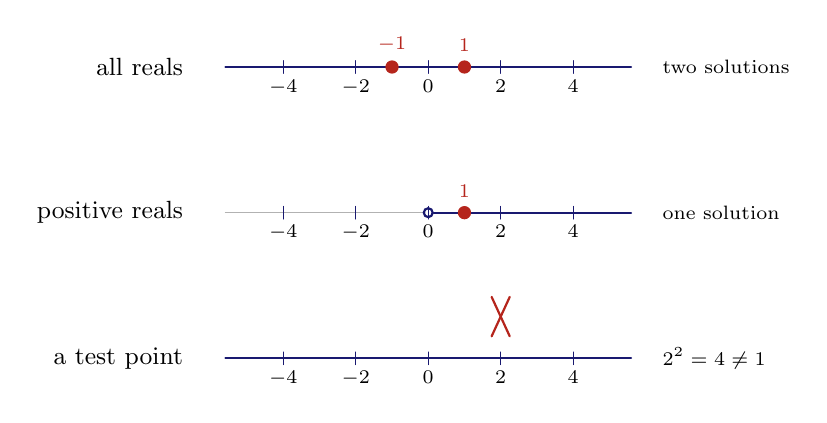
\begin{tikzpicture}[x=0.46cm,y=1cm,line cap=round]
  \def\ocaxislabels{%
    \foreach \n in {-4,-2,0,2,4}{%
      \draw[MidnightBlue] (\n,0.08) -- (\n,-0.08);
      \node[below=1pt,font=\scriptsize,text=black] at (\n,0) {$\n$};}}
  \begin{scope}[yshift=0cm]
    \node[anchor=east,font=\small,align=right,text=black] at (-6.5,0) {all reals};
    \draw[MidnightBlue,thick] (-5.6,0) -- (5.6,0);
    \ocaxislabels
    \fill[BrickRed] (-1,0) circle (2.4pt);
    \fill[BrickRed] (1,0) circle (2.4pt);
    \node[above=2pt,font=\scriptsize,BrickRed] at (-1,0) {$-1$};
    \node[above=2pt,font=\scriptsize,BrickRed] at (1,0) {$1$};
    \node[anchor=west,font=\scriptsize,align=left,text=black] at (6.2,0) {two solutions};
  \end{scope}
  \begin{scope}[yshift=-1.85cm]
    \node[anchor=east,font=\small,align=right,text=black] at (-6.5,0) {positive reals};
    \draw[gray!60] (-5.6,0) -- (0,0);
    \draw[MidnightBlue,thick] (0.15,0) -- (5.6,0);
    \draw[MidnightBlue,thick] (0,0) circle (1.6pt);
    \fill[white] (0,0) circle (1.0pt);
    \ocaxislabels
    \fill[BrickRed] (1,0) circle (2.4pt);
    \node[above=2pt,font=\scriptsize,BrickRed] at (1,0) {$1$};
    \node[anchor=west,font=\scriptsize,align=left,text=black] at (6.2,0) {one solution};
  \end{scope}
  \begin{scope}[yshift=-3.7cm]
    \node[anchor=east,font=\small,align=right,text=black] at (-6.5,0) {a test point};
    \draw[MidnightBlue,thick] (-5.6,0) -- (5.6,0);
    \ocaxislabels
    \draw[BrickRed,thick] (1.75,0.28) -- (2.25,0.78);
    \draw[BrickRed,thick] (2.25,0.28) -- (1.75,0.78);
    \node[anchor=west,font=\scriptsize,align=left,text=black] at (6.2,0) {$2^2=4\neq 1$};
  \end{scope}
\end{tikzpicture}
